% \iffalse
\let\negmedspace\undefined
\let\negthickspace\undefined
\documentclass[journal,12pt,twocolumn]{IEEEtran}
\usepackage{cite}
\usepackage{amsmath,amssymb,amsfonts,amsthm}
\usepackage{algorithmic}
\usepackage{graphicx}
\usepackage{textcomp}
\usepackage{xcolor}
\usepackage{txfonts}
\usepackage{listings}
\usepackage{enumitem}
\usepackage{mathtools}
\usepackage{gensymb}
\usepackage{comment}
\usepackage[breaklinks=true]{hyperref}
\usepackage{tkz-euclide} 
\usepackage{listings}
\usepackage{gvv}                                        
\def\inputGnumericTable{}                                 
\usepackage[latin1]{inputenc}                                
\usepackage{color}                                            
\usepackage{array}                                            
\usepackage{longtable}                                       
\usepackage{calc}                                             
\usepackage{multirow}                                         
\usepackage{hhline}                                           
\usepackage{ifthen}                                           
\usepackage{lscape}
\usepackage{siunitx}
\usepackage{flushend}
\usepackage[siunitx]{circuitikz}
\usepackage{caption}

\newtheorem{theorem}{Theorem}[section]
\newtheorem{problem}{Problem}
\newtheorem{proposition}{Proposition}[section]
\newtheorem{lemma}{Lemma}[section]
\newtheorem{corollary}[theorem]{Corollary}
\newtheorem{example}{Example}[section]
\newtheorem{definition}[problem]{Definition}
\newcommand{\BEQA}{\begin{eqnarray}}
	\newcommand{\EEQA}{\end{eqnarray}}
\newcommand{\define}{\stackrel{\triangle}{=}}
\theoremstyle{remark}
\newtheorem{rem}{Remark}
\begin{document}
	
	\bibliographystyle{IEEEtran}
	\vspace{3cm}
	
	\title{Fibonacci sequence}
	\author{EE22BTECH11052 - Sujal Gupta$^{*}$% <-this % stops a space
	}
	\maketitle
	%\newpage
	\bigskip
	
	\renewcommand{\thefigure}{\theenumi}
	\renewcommand{\thetable}{\theenumi}
	
	
	\vspace{0.2cm}
	\linespread{1.1}
	
	
	\begin{table}[htbp]
	\centering
	\noindent
	\fontsize{10}{15}\selectfont {
		\resizebox{0.5\textwidth}{!}{%
			\begin{tabular}{|c @{\hspace{5pt}\vline}c @{\hspace{8pt}\vline}c@{\hspace{5pt}}|}
				\hline
				\textbf{{Parameter}} &
				\textbf{{\hspace{5pt} Value}} &
				\textbf{{\hspace{2pt} Description}}\\
				\hline
				$y(n)$ & \hspace{2pt} $y(n)$ = $y(n-1)$ + $y(n-2)$  & $(n)^{th}$ term \\
				\hline
				$x(0)$ & 1 & 1$^{st}$ term \\
				\hline
				$x(1)$ & 1 & 2$^{nd}$ term \\
				\hline
			\end{tabular}
	} }
	
	\caption*{Input Table}
	
\end{table}
		
	\begin{align}
	y(0)&=y(-1)+y(-2)=1\\
	y(1)&=y(0)+y(-1)=1
	\end{align}
	Hence,
	\begin{align}
	y(-2)&=1\\
	y(-1)&=0
	\end{align}
	
	
	Applying one sided $z$ transform and considering the initial conditions,
	
	\begin{align}
		Y^{+}\brak z	&= z^{-1} Y^{+}\brak z + y(-1) + z^{-2}Y^{+}\brak z + y(-2) + z^{-1}y(-1) \\
		 		&= \dfrac{1}{1 - z^{-1} - z^{-2}}  \\
		 		&= \dfrac{1}{(1 - \alpha z^{-1})(1 - \beta z^{-1})}				
	\end{align}

	
	Where, \begin{align}\alpha = \dfrac{1 +\sqrt{5}}{2} \\ \beta = \dfrac{1 -\sqrt{5}}{2}\end{align}
	Using partial fractions,
	
	\begin{align}
		X(z) = \dfrac{\alpha}{(\alpha - \beta)} \dfrac{1}{(1 - \alpha z^{-1})} - \dfrac{\beta}{(\alpha - \beta)} \dfrac{1}{(1 - \beta z^{-1})}
	\end{align}
	\begin{align}a^n u(n)
	\xleftarrow[]{\hspace{0.4cm}{\mathcal{Z}}\hspace{0.1cm}}\xrightarrow[]{}
	\dfrac{1}{1 - a z^{-1}}  |z| \hspace{0.1cm}> \hspace{0.1cm} \lvert \hspace{0.1cm} a \hspace{0.1cm} \rvert
	\end{align}

	
	Substituting this result,
	\begin{align}
		x(n) &= \dfrac{\alpha}{(\alpha - \beta)} ({\alpha}^n u(n)) - \dfrac{\beta}{(\alpha - \beta)} ({\beta}^n u(n)) \\
	&= \dfrac{\alpha^{n+1} - \beta^{n+1} }{\alpha - \beta} u(n)\\
	 &= \dfrac{(1 + \sqrt{5})^{n+1} - (1 - \sqrt{5})^{n+1} }{2^{n+1} \sqrt{5}}u(n)
	\end{align}
	
	\newpage
	
	\begin{figure}[htbp]
		\centering
		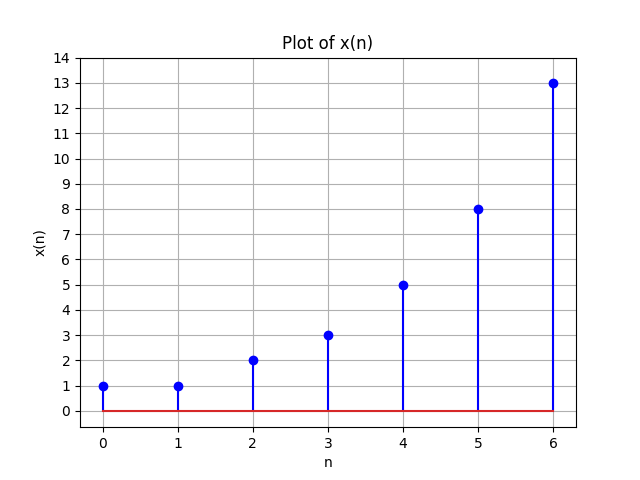
\includegraphics[width=0.5\textwidth]{figs/fig1.png}
		\label{fibonacci}
		\caption*{\hspace{2cm} (a) Plot of $x(n)$ $vs$ $n$}
	\end{figure}
	

\end{document}
